\section{Auswertung}
\label{sec:Auswertung}

Zur Bestimmung der Zeitkonstanten wird im Folgenden die Entladekurve des Kondensators betrachtet.
Die dazu aufgenommenen Messwerte sind in \autoref{tab:Entladekurve} aufgetragen. 

\begin{table}[H]
  \centering
  \caption{Entladekurve einer RC-Schwingkreises.}
  \label{tab:Entladekurve}
  \begin{tabular}{S S}
    \toprule
    {$T \mathbin{/} \unit{\milli\second} $} &  {$ U \mathbin{/} \unit{\milli\volt}$} \\
    \midrule
            0      &         18     \\
            1      &         12     \\
            2      &         7.5    \\
            3      &         5      \\
            4      &         3      \\
            5      &         2      \\
            6      &         1.5    \\
            7      &         1      \\
            8      &         0.5    \\
            9      &         0.25   \\
            10     &         0      \\
  \end{tabular}
\end{table}

Über die in \autoref{fig:ausgleichsa)} dargestellte Ausgleichsrechnung lässt sich nun die Zeitkonstante $τ = \dfrac{1}{RC}$ ermitteln.
Die Ausgleichsrechnung folgt dabei der Funktionsvorschrift
\begin{equation*}
  \ln(\frac{U_C}{U_0}) = -\frac{1}{RC} t + b \,.
\end{equation*}

\begin{figure}[H]
  \centering
  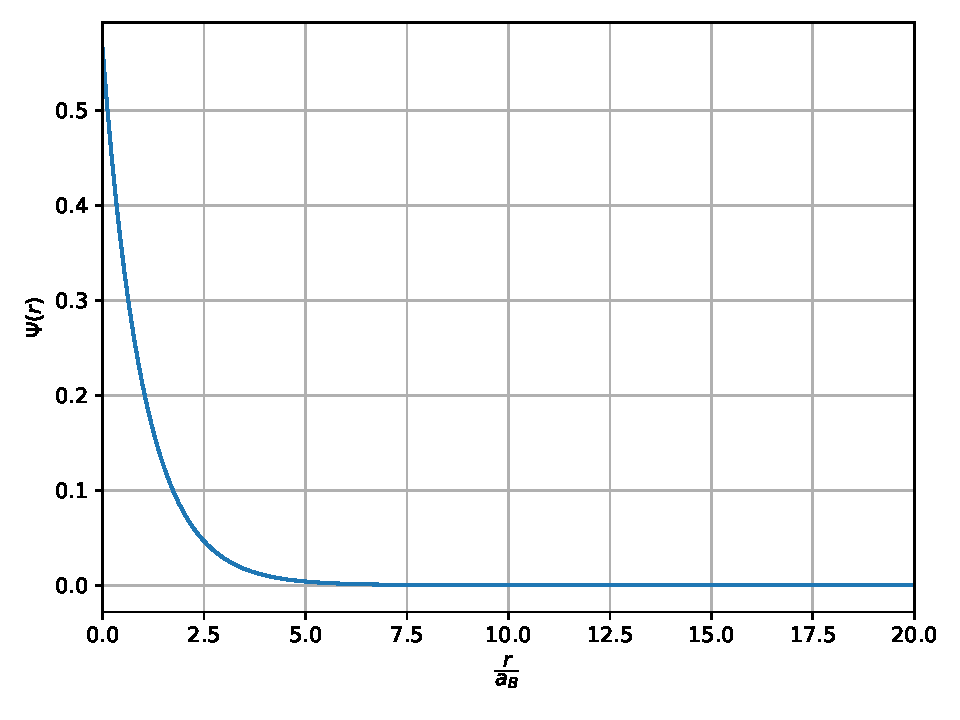
\includegraphics{build/Graph_a.pdf}
  \caption{Halblogarithmische Darstellung der Messwerte und Ausgleichskurve.}
  \label{fig:ausgleichsa)}
\end{figure}

Die Parameter ergeben sich damit zu 
\begin{equation*}
  RC = (0,00221 \pm 0,00007) \,\unit{\second}
\end{equation*} 

\begin{equation*}
  b = 0,06 \pm 0,08 \,.
\end{equation*}

Anschließend wurde die Amplitude $U$ sowie die Phasenverschiebung nach \autoref{fig:phasenversch} gemessen.
Für die Wertepaare $(a,b)$ wurde nur dann die Periodendauer $b$ gemessen, wenn die Phasenverschiebung $\varphi \neq 0$ war.

\begin{table}[H]
  \centering
  \caption{Messwerte zur Amplitude und Phasenverschiebung des RC-Schwingkreises.}
  \label{tab:phasenver}
  \begin{tabular}{S S S S}
    \toprule
    {$f \mathbin{/} \unit{\hertz}$} & {$U \mathbin{/} \unit{\volt} $} & {$a \mathbin{/} \unit{\micro\meter} $} & {$b \mathbin{/} \unit{\micro\meter} $} \\
    \midrule
    40          & 8.5                 & 0                   & {-}        \\
    50          & 9                   & 0                   & {-}        \\
    80          & 8.5                 & 0                   & {-}        \\
    160         & 7.5                 & 0                   & {-}        \\
    300         & 8                   & 0                   & {-}        \\
    600         & 7.5                 & 0                   & {-}        \\
    1000        & 8                   & 0                   & {-}        \\
    1500        & 8                   & 0                   & {-}        \\
    2000        & 7                   & 0                   & {-}        \\
    2500        & 6.4                 & 0                   & {-}        \\
    3000        & 5.6                 & 0                   & {-}        \\
    4000        & 4.8                 & 0                   & {-}        \\
    5000        & 4                   & 0                   & {-}        \\
    6000        & 3.2                 & 0                   & {-}        \\
    7000        & 3                   & 0                   & {-}        \\
    10000       & 2.2                 & 4                   & 40         \\
    11000       & 2                   & 4.6                 & 40         \\
    15000       & 1.6                 & 2                   & 40         \\
    20000       & 1.2                 & 1.5                 & 22.5       \\
    22000       & 1                   & 5                   & 20         \\
    25000       & 0.8                 & 2.5                 & 20         \\
    30000       & 0.8                 & 0                   & 17         \\
    40000       & 0.4                 & 0                   & 12         \\
  \end{tabular}
\end{table}

Die Ausgleichskurve in \autoref{fig:ausgleichsb)} wurde dabei nach \eqref{eq:amplitudendingens} mit der Form
\begin{equation*}
  U(\omega) = \frac{U_0}{\sqrt{1 + \omega^2 R^2 C^2}}
\end{equation*}
bestimmt.

\begin{figure}[H]
  \centering
  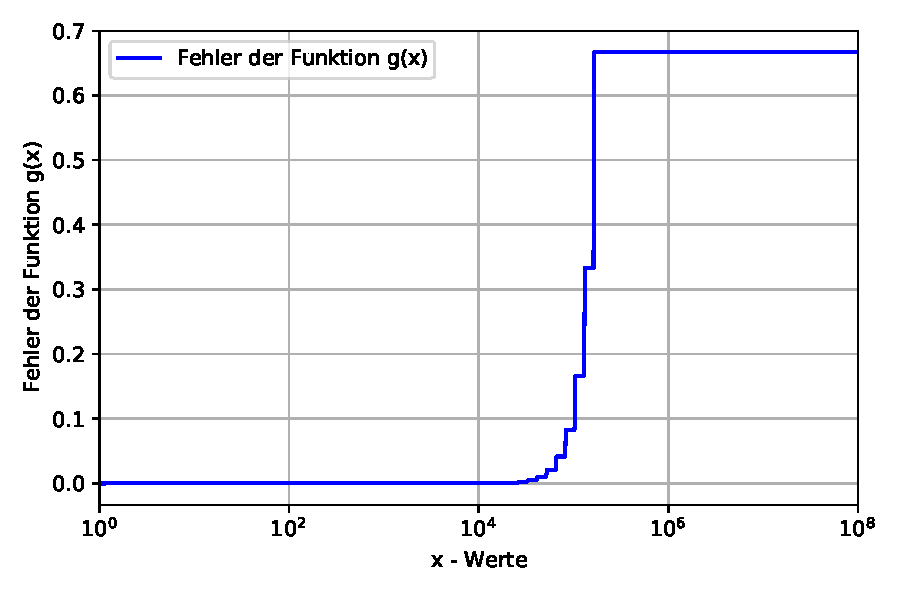
\includegraphics{build/Graph_b.pdf}
  \caption{Messwerte der Amplitude und Ausgleichskurve in Abhängigkeit von der Frequenz.}
  \label{fig:ausgleichsb)}
\end{figure}

Dabei ergeben sich 
\begin{equation*}
  U_0 = 8,334 \,\unit{\volt}
\end{equation*}
und
\begin{equation*}
  RC = (0,018897 \pm 0,000017) \,\unit{\second} \,.
\end{equation*}

Die Phasenverschiebungen seien nun in \autoref{fig:phasenverschiebungen} dargestellt.

\begin{table}[H]
  \centering
  \caption{Phasenverschiebung $\varphi$ der Generator- und Kondensatorspannung.}
  \label{fig:phasenverschiebungen}
  \begin{tabular}{S S}
    \toprule
    {$ν \mathbin{/} \unit{\hertz} $} &  {$ \varphi \mathbin{/} rad$} \\
    \midrule
    40    & 0     \\ 
    50    & 0     \\ 
    80    & 0     \\ 
    160   & 0     \\ 
    300   & 0     \\ 
    600   & 0     \\ 
    1000  & 0     \\ 
    1500  & 0     \\ 
    2000  & 0     \\ 
    2500  & 0     \\ 
    3000  & 0     \\ 
    4000  & 0     \\ 
    5000  & 0     \\ 
    6000  & 0     \\ 
    7000  & 0     \\ 
    10000 & 0.628 \\
    11000 & 0.723 \\
    15000 & 0.314 \\
    20000 & 0.419 \\
    22000 & 1.571 \\
    25000 & 0.785 \\
    30000 & 0     \\
    40000 & 0     \\
  \end{tabular}
\end{table}

Die Frequenzabhängigkeit der Phasenverschiebung sei in \autoref{fig:frequpha} aufgetragen.

\begin{figure}[H]
  \centering
  \includegraphics{build/Graph_b2.pdf}
  \caption{Frequenzabhängigkeit der Phasenverschiebung und Ausgleichskurve.}
  \label{fig:frequpha}
\end{figure}

Die Ausgleichsrechnung wurde dabei nach \eqref{eq:arctan} durchgeführt.

Es ergibt sich
\begin{equation*}
  RC = (2,570 \pm 1,380) \cdot 10^{-5} \, \unit{\second} \,.
\end{equation*}

Abschließend sei in \autoref{fig:polarplot} der Polarplot der Phasenverschiebung gegen die Spannung dargestellt.

\begin{figure}
  \centering
  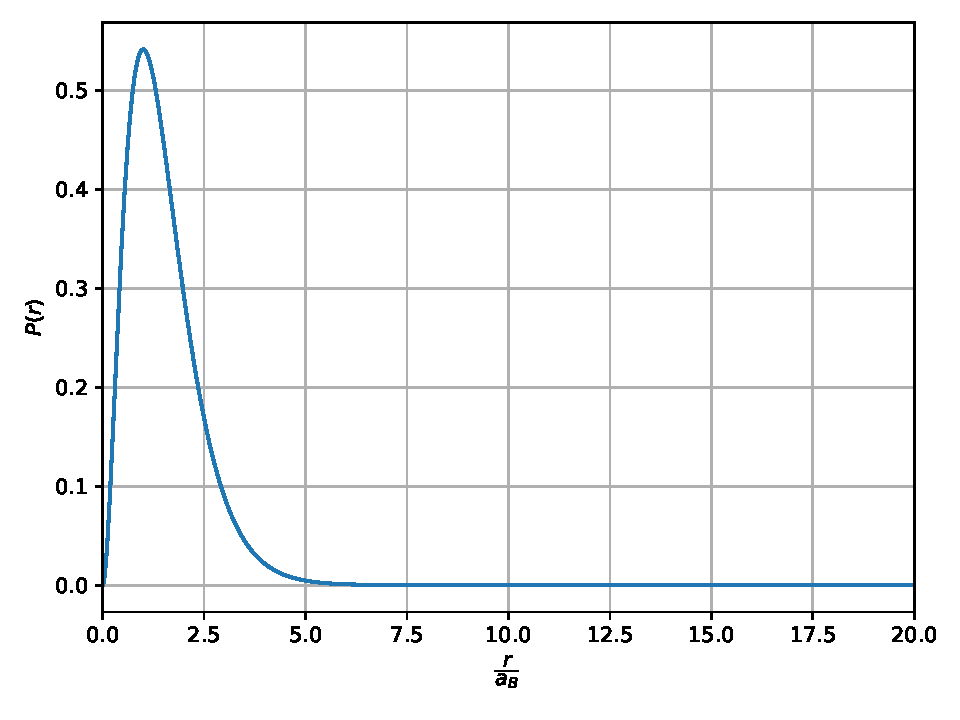
\includegraphics{build/Graph_c.pdf}
  \caption{Polarplot der Messdaten.}
  \label{fig:polarplot}
\end{figure}